\subsection{Online Clustering}
\label{subsec:4c_online_clustering}

\subsubsection{Design}
\label{subsubsec:4c_design}

Detecting events in a stream of news articles will be achieved by using an online clustering approach.
An event is described by the occurrence of multiple news articles about the same story.
The events of interest for this application are the discovery of new stories and the extension of existing stories.
Thus we define our two types of events as follows:

\begin{itemize}
    \item New event: A new cluster of news articles appears in the data stream, which write about the same story.
    \item Event extended: An existing story is extended by additional news articles.
\end{itemize}

HDBSCAN will be applied as the clustering method,
using the optimal settings discovered in the clustering method evaluation.
Additional preprocessing of news articles before clustering is going to be explored
as part of evaluation as well and will be implemented accordingly for the online clustering.

The clustering will be done in batches over time, since HDBSCAN only supports static data sets.
Events are detected by comparing clusters from successive batches.
\figref{fig:timeline} illustrates this with three batches,
where the resulting clusters from batch $t$ will be compared with the previous result from batch $t - 1$,
while batch $t - 1$ was previously compared with batch $t - 2$.

In this example, each batch only contains samples from a limited time period,
where $\triangle t$ stands for the time period between batches.
Since a batch does not contain the full set of samples, we have to consider the overlap between batches.
The size of the overlap is essential to find similar clusters from different batches.
If a similar cluster already exists in the previous batch,
the differences between these clusters are detected as a change in an existing event.
If no pair exists for a cluster from a current batch, this cluster will be regarded as a new event.
The similarity between clusters is based on the same assumptions
as for the scoring function described in \subsubsecref{subsubsec:4b_scoring_function}.

\begin{figure}[h]
    \centering

    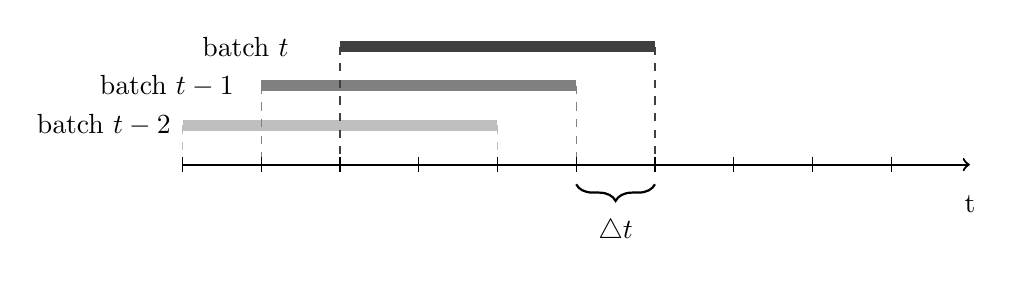
\begin{tikzpicture}[scale=1]

        \draw[lightgray, line width=4pt] (0,.5) -- (4,.5);
        \draw[lightgray, dashed] (0,.5) -- (0,0);
        \draw[lightgray, dashed] (4,.5) -- (4,0);
        \node[align=right] at (-1,.5) {batch $t - 2$};

        \draw[gray, line width=4pt] (1,1) -- (5,1);
        \draw[gray, dashed] (1,1) -- (1,0);
        \draw[gray, dashed] (5,1) -- (5,0);
        \node[align=right] at (-.2,1) {batch $t - 1$};

        \draw[darkgray, line width=4pt] (2,1.5) -- (6,1.5);
        \draw[darkgray, dashed] (2,1.5) -- (2,0);
        \draw[darkgray, dashed] (6,1.5) -- (6,0);
        \node[align=right] at (0.8,1.5) {batch $t$};

        \node[align=center] at (5.5,-0.85) {$\triangle t$};
        \node[align=center] at (10,-0.5) {t};

        \draw [thick,->] (0,0) -- (10,0);
        \foreach \x in {0,...,9} \draw (\x,0.1) -- (\x,-0.1);

        \draw [thick,decorate,decoration={brace,amplitude=6pt,raise=0pt,mirror}] (5,-0.25) -- (6,-0.25);

        \end{tikzpicture}

    \caption{Timeline showing the sliding window approach.}
    \label{fig:timeline}
\end{figure}

The overlap between batches depends on the batch size and the number of new samples in $\triangle t$.
A high volume of incoming samples combined with a small batch size
would result in an overlap too small to find pairs of clusters.
All clusters from the current batch would be detected as new in such case.
To decrease the negative impact on the event detection by peaks in the data stream,
we need a batch size which grows accordingly.
The ideal batch size provides enough overlap between batches to find pairs of clusters
and is small enough to allow efficient processing.
We explore three different methods for determining the ideal batch size:

\begin{enumerate}
    \item \textbf{Fixed size}: The first method uses a fixed batch size,
          where each batch processes the most recent \textit{n} samples.
          This makes the clustering unstable against sudden peaks in the volume of incoming data,
          but we consider this method as an useful benchmark for the dynamic methods.
    \item \textbf{Size by hours}: This method uses a dynamic batch size
          by loading the samples from the last \textit{n} hours.
          This enables the batch size to increase and decrease with the volume of the data stream.
          The number of samples will be limited by an upper bound,
          to keep the space and time consumption of the clustering method reasonable.
    \item \textbf{Size by incoming data}: This method defines the batch size relative to the incoming stream of data.
          We count the number of new samples since the last batch and multiply it by a predefined factor.
          For example, if we want the new samples to be 1\%
          of the overall clustering, we define the factor as 100.
          The batch size will be limited by a lower and an upper bound.
          The lower bound prevents the overlap between batches from getting too small.
          The upper bound is based on the same reasoning as mentioned in the previous method.
\end{enumerate}

The evaluation will use the MP-Score to measure the precision of the event detection,
since our model represents events as clusters.
True events can be extracted directly from the ground truth based on news articles from two successive batches.

\subsubsection{Implementation}
\label{subsubsec:4c_implementation}

The online clustering implemented for this thesis does not operate in a true online setting,
but rather in a simulated data stream over time.
The simulated approach allows us to directly compare the resulting events
with the ground truth and thus evaluate different settings.
The implementation was done with Python and runs in a dockerized environment similar to the evaluation framework.

The detection of events relies on comparing clusters between successive batches. 
We apply \gls{lsh}\cite{alex2015practical} to find clusters most similar to each other.
In its essence, \gls{lsh} is an efficient way to find similar documents,
which does not require to calculate the similarity between each possible pair of documents. 
The implementation for \gls{lsh} is provided by the datasketch library\cite{eric_zhu_2017_290602}.

Once we have found pairs of clusters which represent the same story, detecting events becomes trivial.
For each pair we subtract the cluster from the previous batch from the current cluster.
The resulting set contains all news articles, which are only present in the current cluster.
These articles are then summarized as a change of an existing event. 
If the previous batch did not contain any similar clusters for a cluster from the current batch, 
the cluster is considered as a new event.

Since events are clusters of news articles themselves,
we apply the MP-Score to measure the precision of detected events. 
Calculating the score has a time complexity of $O(n^2)$, but since the application runs on a simulated timeline and the scoring is only part of the evaluation,
time complexity is a minor concern in this case.

\paragraph{CLI}
The application provides a command line interface to run the simulation with different parameters
such as the start date, number of days to run and the batch size.

\begin{lstlisting}[caption=Command line interface for the online clustering., label={lst:cli_online_clustering}]
usage: online_clustering.py [-h] [--verbose] [--persist_in_db] 
                            [--rows ROWS] [--hours HOURS] 
                            [--factors FACTORS] --date DATE
                            [--run_n_days RUN_N_DAYS] 
                            [--threshold THRESHOLD]

Run the batchwise clustering over a simulated stream of news articles.

optional arguments:
-h, --help              show this help message and exit
--verbose               default: False
--persist_in_db         default: False
--rows ROWS             numbers of samples to process per batch
--hours HOURS           numbers of hours to load samples
--factors FACTORS       factor to use for relative batch sizes
--date DATE             start date
--run_n_days RUN_N_DAYS number of days to run the batchwise clustering
                        default: 1
--threshold THRESHOLD   similarity threshold for cluster matching
                        default: 0.75

\end{lstlisting}
